107. \begin{figure}[ht!]
\center{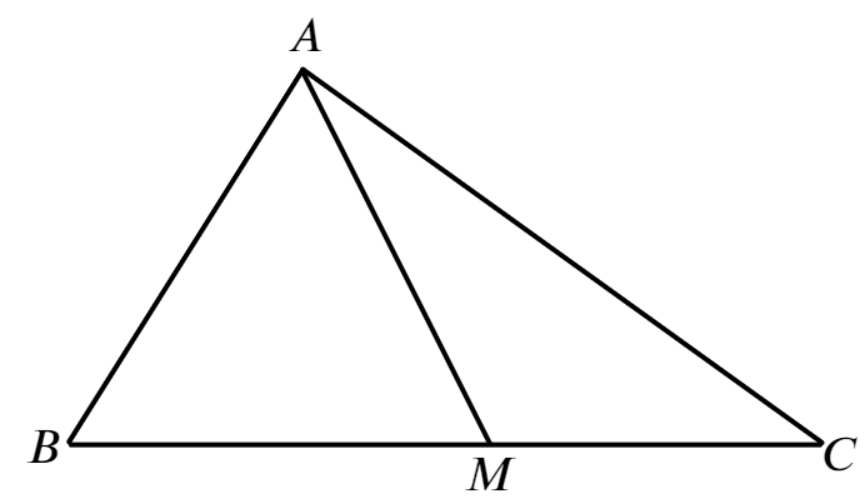
\includegraphics[scale=0.35]{g9-107.png}}
\end{figure}\\
Найдём $BM=\cfrac{5}{9}\cdot18=10.$ По теореме косинусов для треугольника $ABC$ имеем равенства $15^2=12^2+18^2-2\cdot12\cdot18\cos(\angle B),\ \cos(\angle B)=\cfrac{9}{16}.$ По теореме косинусов для треугольника $ABM$ получим $AM^2=12^2+10^2-2\cdot12\cdot10\cdot\cfrac{9}{16}=109,\ AM=\sqrt{109}.$\\
